%----------------------------------------------------------------------------------------
%	PACKAGES AND OTHER DOCUMENT CONFIGURATIONS
%----------------------------------------------------------------------------------------

\documentclass[15pt]{article}

\usepackage[margin=1in]{geometry}
\usepackage{amsfonts}
\usepackage{minted}
\usepackage[utf8]{inputenc}
\usepackage{usecases}
\usepackage{CJKutf8}
\usepackage{booktabs}
\usepackage[toc,page]{appendix}
\usepackage{color,soul}
\usepackage{listings}
\usepackage{algorithm}% http://ctan.org/pkg/algorithm
\usepackage{algpseudocode}% http://ctan.org/pkg/algorithmicx
\lstset{escapechar=§}
\usepackage{siunitx}
\usepackage[norndcorners,customcolors]{hf-tikz}
\hfsetbordercolor{yellow}
\hfsetfillcolor{yellow}
\usepackage{graphicx}
\usepackage[export]{adjustbox} 
\usepackage{lipsum}%% a garbage package you don't need except to create examples.
\usepackage{fancyhdr}
\pagestyle{fancy}
\lhead{Xueying Li 40036265}
\rhead{SOEN 6011 Project-F3-D2-2}
\usepackage{listings}
\usepackage{color}
\definecolor{dkgreen}{rgb}{0,0.6,0}
\definecolor{gray}{rgb}{0.5,0.5,0.5}
\definecolor{mauve}{rgb}{0.58,0,0.82}
    
\lstset{frame=tb,
  language=Java,
  aboveskip=3mm,
  belowskip=3mm,
  showstringspaces=false,
  columns=flexible,
  basicstyle={\small\ttfamily},
  numbers=none,
  numberstyle=\tiny\color{gray},
  keywordstyle=\color{blue},
  commentstyle=\color{dkgreen},
  stringstyle=\color{mauve},
  breaklines=true,
  breakatwhitespace=true,
  tabsize=3
}
\lstset{language=Java}
\usepackage{subcaption}
\usepackage{makecell} 
\usepackage{graphicx}
\usepackage[utf8]{inputenc}

% document structure and custom commands

\usepackage{amsmath,amsfonts,stmaryrd,amssymb} % Math packages

\usepackage{enumerate} % Custom item numbers for enumerations

\usepackage[ruled]{algorithm2e} % Algorithms
\usepackage{fontawesome}

\usepackage[framemethod=tikz]{mdframed} % Allows defining custom boxed/framed environments
    
\usepackage{listings} % File listings, with syntax highlighting
\lstset{
	basicstyle=\ttfamily, % Typeset listings in monospace font
}

\usepackage{geometry} % Required for adjusting page dimensions and margins

\geometry{
	paper=a4paper, % Paper size, change to letterpaper for US letter size
	top=2.5cm, % Top margin
	bottom=3cm, % Bottom margin
	left=2.5cm, % Left margin
	right=2.5cm, % Right margin
	headheight=14pt, % Header height
	footskip=1.5cm, % Space from the bottom margin to the baseline of the footer
	headsep=1.2cm, % Space from the top margin to the baseline of the header
	%showframe, % Uncomment to show how the type block is set on the page
}


\usepackage[utf8]{inputenc} % Required for inputting international characters
\usepackage[T1]{fontenc} % Output font encoding for international characters

\usepackage{XCharter} % Use the XCharter fonts

% Usage:
% \begin{commandline}
%	\begin{verbatim}
%		$ ls
%		
%		Applications	Desktop	...
%	\end{verbatim}
% \end{commandline}

\mdfdefinestyle{commandline}{
	leftmargin=10pt,
	rightmargin=10pt,
	innerleftmargin=15pt,
	middlelinecolor=black!50!white,
	middlelinewidth=2pt,
	frametitlerule=false,
	backgroundcolor=black!5!white,
	frametitle={Command Line},
	frametitlefont={\normalfont\sffamily\color{white}\hspace{-1em}},
	frametitlebackgroundcolor=black!50!white,
	nobreak,
}

% Define a custom environment for command-line snapshots
\newenvironment{commandline}{
	\medskip
	\begin{mdframed}[style=commandline]
}{
	\end{mdframed}
	\medskip
}

% Usage:
% \begin{file}[optional filename, defaults to "File"]
%	File contents, for example, with a listings environment
% \end{file}

\mdfdefinestyle{file}{
	innertopmargin=1.6\baselineskip,
	innerbottommargin=0.8\baselineskip,
	topline=false, bottomline=false,
	leftline=false, rightline=false,
	leftmargin=2cm,
	rightmargin=2cm,
	singleextra={%
		\draw[fill=black!10!white](P)++(0,-1.2em)rectangle(P-|O);
		\node[anchor=north west]
		at(P-|O){\ttfamily\mdfilename};
		%
		\def\l{3em}
		\draw(O-|P)++(-\l,0)--++(\l,\l)--(P)--(P-|O)--(O)--cycle;
		\draw(O-|P)++(-\l,0)--++(0,\l)--++(\l,0);
	},
	nobreak,
}

% Define a custom environment for file contents
\newenvironment{file}[1][File]{ % Set the default filename to "File"
	\medskip
	\newcommand{\mdfilename}{#1}
	\begin{mdframed}[style=file]
}{
	\end{mdframed}
	\medskip
}


% Usage:
% \begin{question}[optional title]
%	Question contents
% \end{question}

\mdfdefinestyle{question}{
	innertopmargin=1.2\baselineskip,
	innerbottommargin=0.8\baselineskip,
	roundcorner=5pt,
	nobreak,
	singleextra={%
		\draw(P-|O)node[xshift=1em,anchor=west,fill=white,draw,rounded corners=5pt]{%
		Question \theQuestion\questionTitle};
	},
}

\newcounter{Question} % Stores the current question number that gets iterated with each new question

% Define a custom environment for numbered questions
\newenvironment{question}[1][\unskip]{
	\bigskip
	\stepcounter{Question}
	\newcommand{\questionTitle}{~#1}
	\begin{mdframed}[style=question]
}{
	\end{mdframed}
	\medskip
}

% Usage:
% \begin{warn}[optional title, defaults to "Warning:"]
%	Contents
% \end{warn}

\mdfdefinestyle{warning}{
	topline=false, bottomline=false,
	leftline=false, rightline=false,
	nobreak,
	singleextra={%
		\draw(P-|O)++(-0.5em,0)node(tmp1){};
		\draw(P-|O)++(0.5em,0)node(tmp2){};
		\fill[black,rotate around={45:(P-|O)}](tmp1)rectangle(tmp2);
		\node at(P-|O){\color{white}\scriptsize\bf !};
		\draw[very thick](P-|O)++(0,-1em)--(O);%--(O-|P);
	}
}

% Define a custom environment for warning text
\newenvironment{warn}[1][Warning:]{ % Set the default warning to "Warning:"
	\medskip
	\begin{mdframed}[style=warning]
		\noindent{\textbf{#1}}
}{
	\end{mdframed}
}


% Usage:
% \begin{info}[optional title, defaults to "Info:"]
% 	contents
% 	\end{info}

\mdfdefinestyle{info}{%
	topline=false, bottomline=false,
	leftline=false, rightline=false,
	nobreak,
	singleextra={%
		\fill[black](P-|O)circle[radius=0.4em];
		\node at(P-|O){\color{white}\scriptsize\bf i};
		\draw[very thick](P-|O)++(0,-0.8em)--(O);%--(O-|P);
	}
}

% Define a custom environment for information
\newenvironment{info}[1][Info:]{ % Set the default title to "Info:"
	\medskip
	\begin{mdframed}[style=info]
		\noindent{\textbf{#1}}
}{
	\end{mdframed}
}

%Adds "References" to the table of contents
\title{Bibliography management:\\\texttt{thebibliography} environment}


\begin{document}
\begin{CJK*}{UTF8}{gbsn}
% Cover page
{\fontfamily{cmr}\selectfont
\title{ \normalsize \textsc{}
		\\ [2.0cm]
		\LARGE \textbf{\uppercase{
		\\
		SOEN 6011 PROJECT DELIVERY 2-2:\\ REVIEWS of CALCULATOR of FUNCTION 3(CF3) APPLICATION\\}
		\normalsize \today \vspace*{5\baselineskip}}
		}
\date{}

\author{
		Xueying Li 40036265\\ 
		\href{https://github.com/raphealshirley/SOEN6011-PROJECT}
		}

\maketitle
\newpage

\section{Source Code Review}
Code review is systematic examination of computer source code. It is intended to find mistakes overlooked in the initial development phase, improving the overall quality of software\cite{1}.


\subsection{Code Review Methodology}
Main phrases of code review are showing as figure 1a. It includes preparation, execution, assessment and reporting.\\
In this code reviewing process, an inspection was performed to find anomalies and to generate anomalies list though using Java Code Review Checklist\cite{2}.\\
Checklist is an important approach to assist the reviewer to generate a defect list. Utilizing Java Code Review Checklist to review could help evaluate the quality of the java code, and in our reviewing process, quality attributes taken into consideration are clean code, security, performance, static code analysis and error handling.And figure 1b shows all the attributes.

\begin{figure}[ht]
\centering
	\begin{subfigure}{0.49\linewidth}\centering
    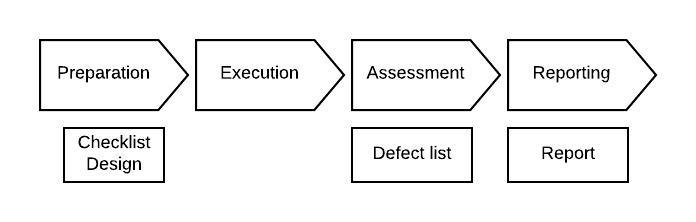
\includegraphics[scale = 0.7]{flow.jpeg}
    \caption{Methodology Phases}\label{fig:figA}
    \end{subfigure}
	\begin{subfigure}{0.49\linewidth}\centering
    	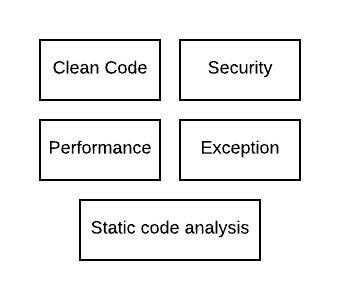
\includegraphics[scale = 0.7]{quality.jpeg}
        \caption{Quality Attributes}\label{fig:figB}
  		\end{subfigure}
\caption{Code Review Methodology} \label{fig:twofigs}
\end{figure}

\subsection{Checklists}
In our review process, a modified java code review check list is used based on\cite{2}. Following gives the modified checklist.
\begin{table}[htp]
\centering
\caption{Checklist for Clean Code}
\begin{tabular}{@{}|l|l|l|@{}}
\toprule
\multicolumn{3}{|c|}{Clean Code}                                         \\ \midrule
Category         & Checklist Item                            & File-Line \\ \midrule
Meaningful Names & Use Intention-Revealing Names             &           \\ \midrule
                 & Pick one word per concept                 &           \\ \midrule
                 & Use Solution/Problem Domain Names         &           \\ \midrule
Classes          & Classes should be small!                  &           \\ \midrule
Functions        & Functions should be small!                &           \\ \midrule
                 & Do one Thing                              &           \\ \midrule
                 & Don't Repeat Yourself (Avoid Duplication) &           \\ \midrule
Comments         & Explain yourself in code                  &           \\ \midrule
Formatting       & Make sure the code formatting is applied  &           \\ \midrule
Exceptions       & Use Exceptions rather than Return codes   &           \\ \midrule
                 & Don't return Null                         &           \\ \bottomrule
\end{tabular}
\end{table}

\begin{table}[htp]
\centering
\caption{Checklist for Security}
\begin{tabular}{@{}|l|l|l|@{}}
\toprule
\multicolumn{3}{|c|}{Security}                                                                                                                                                                                                        \\ \midrule
Category                                                            & Checklist Item                                                                                                                                      & File-Line \\ \midrule
Fundamentals                                                        & Make class final if not being used for inheritance                                                                                                  &           \\ \midrule
                                                                    & Avoid duplication of code                                                                                                                           &           \\ \midrule
                                                                    & Minimize the accessibility of classes and members                                                                                                   &           \\ \midrule
Denial of Service                                                   & \begin{tabular}[c]{@{}l@{}}Input into a system should be checked for valid data size\\ and range\end{tabular}                                       &           \\ \midrule
                                                                    & Release resources (Streams, Connections, etc) in all cases                                                                                          &           \\ \midrule
\begin{tabular}[c]{@{}l@{}}Confidential \\ Information\end{tabular} & \begin{tabular}[c]{@{}l@{}}Purge sensitive information from exceptions (exposing file \\ path, internals of the system, configuration)\end{tabular} &           \\ \midrule
Input Validation                                                    & Validate inputs (for valid data, size, range, boundary conditions, etc)                                                                             &           \\ \bottomrule
\end{tabular}
\end{table}

\begin{table}[htp]
\centering
\caption{Checklist for performance}
\begin{tabular}{@{}|l|l|l|@{}}
\toprule
\multicolumn{3}{|c|}{Perfromance}                                                                                                                                                                                                     \\ \midrule
Category                                                            & Checklist Item                                                                                                                                      & File-Line \\ \midrule
Creating and Destroying Objects                                     & Avoid creating unnecessary objects                                                                                                                  &           \\ \midrule
                                                                    & Beware the performance of string concatenation                                                                                                      &           \\ \midrule
                                                            
\end{tabular}
\end{table}

\begin{table}[htp]
\centering
\caption{Checklist for Exception Handling}
\begin{tabular}{@{}|l|l|l|@{}}
\toprule
\multicolumn{3}{|c|}{Exception Handling}                                                                                                                            \\ \midrule
Category   & Checklist Item                                                                                                                             & File-Line \\ \midrule
Exceptions & \begin{tabular}[c]{@{}l@{}}Use checked exceptions for recoverable conditions and \\ runtime exceptions for programming errors\end{tabular} &           \\ \midrule
           & Don't ignore exceptions                                                                                                                    &           \\ \bottomrule
\end{tabular}
\end{table}

\begin{table}[htp]
\centering
\caption{Checklist for Static Code Analysis}
\begin{tabular}{@{}|l|l|l|@{}}
\toprule
\multicolumn{3}{|c|}{Static Code Analysis}                                                          \\ \midrule
Category             & Checklist Item                                                   & File-Line \\ \midrule
Static Code Analysis & Check static code analyzer report for the classes added/modified &           \\ \bottomrule
\end{tabular}
\end{table}

\subsection{Assessment}
\subsubsection{Defect List}
Following table gives a compete defect list.
\begin{table}[htp]
\centering
\caption{Defect list}
\begin{tabular}{@{}|l|l|l|@{}}
\toprule
\multicolumn{3}{|c|}{Defect List}                          \\ \midrule
Quality Attribute-Category         & Checklist Item                            & File-Line \\ \midrule
Clean Code-Meaningful Names & Use Intention-Revealing Names             & log-16    \\ \midrule
Security-Fundamentals & Make class final if not being used for inheritance             & log-5    \\ \midrule

\end{tabular}
\end{table}

\subsubsection{Checkstyle Result}
In this application, Checkstyle\cite{3} is used for course code quality checking. Checktyle is a static code analysis tool used in software development for checking if Java source code complies with coding rules\cite{3}.Coding standards for checking is google coding standard according to Google Java Style Guide\cite{4}.The final result is \textit{Checkstyle found no problems in the file(s)}.\\

\subsection{Report}
A checklist-based infection source code reviewing is implemented. In overall, source code is proved to be relatively clean, secure, good-performed with good exception handling based on checklists. Although naming was not perfect, the output of checkstyle shows its good code style. Another small defect is that class would be more secure if is made final.
\section{Testing}
Unit Testing is implemented using Junit, and computer environment is Junit4 and Java 1.8. IDE is intellij.
\subsection{Overall Test Results}
All tests passed. And the calculation accuracy is all over 99.99 percents. 100 percent of the test is OK. There are no bugs to be reported.Following gives all OK tests which covers all the test cases.\\
In overall, test-ability is ensured as the test environment worked well. All test cases passed with result of OK and the accuracy was ensured. \\
\subsection{Detailed Test Report}
Following table 7 gives all the test cases with detailed infomation.
\begin{table}[!htp]
\centering
\caption{Test Results - OK}
\begin{tabular}{@{}|l|l|l|l|l|l|l|@{}}
\toprule
\multicolumn{7}{|c|}{Test Result-OK}   \\ \midrule
\multicolumn{1}{|c|}{ID} & \multicolumn{1}{c|}{Test Method} & \multicolumn{1}{c|}{Test Date} & \multicolumn{1}{c|}{Input} & \multicolumn{1}{c|}{Expected Output} & \multicolumn{1}{c|}{Actual Output} & \multicolumn{1}{c|}{\begin{tabular}[c]{@{}c@{}}State\\ (Pass/Fail)\end{tabular}} \\ \midrule
1                        & LogGamma                         & 30.Jul.2019                    & 1                          & 0                                    & 0                                  & Pass                                                                             \\ \midrule
2                        &                                  & 30.Jul.2019                    & 1.53                       & -0.1192705602                        & -0.1192705602                      & Pass                                                                             \\ \midrule
3                        &                                  & 30.Jul.2019                    & 10.75                      & 14.51947223                          & 14.51947223                        & Pass                                                                             \\ \midrule
4                        &                                  & 30.Jul.2019                    & 100.65                     & 362.1264291                          & 362.1264291                        & Pass                                                                             \\ \midrule
5                        &                                  & 30.Jul.2019                    & 1.82E80                    & -0.06523734313                       & -0.06523734313                     & Pass                                                                             \\ \midrule
6                        & Gamma                            & 30.Jul.2019                    & 6                          & 120                                  & 120                                & Pass                                                                             \\ \midrule
7                        &                                  & 30.Jul.2019                    & 4.000001                   & 6.000007537                          & 6.000007537                        & Pass                                                                             \\ \midrule
8                        &                                  & 30.Jul.2019                    & -3.2                       & 0.689056412                          & 0.689056412                        & Pass                                                                             \\ \midrule
9                        &                                  & 30.Jul.2019                    & -0.00001                   & -100,000.5772                        & -100,000.5772                      & Pass                                                                             \\ \midrule
10                       &                                  & 30.Jul.2019                    & -42.232                    & -1.40581004E-51                      & -1.40581004E-51                    & Pass                                                                             \\ \midrule
11                       &                                  & 30.Jul.2019                    & -242.232                   & -5.5611603E-474                      & -5.5611603E-474                    & Pass                                                                             \\ \midrule
12                       &                                  & 30.Jul.2019                    & 100.87                     & 5.125761144E+157                     & 5.125761144E+157                   & Pass                                                                             \\ \midrule
13                       &                                  & 30.Jul.2019                    & -20.87                     & -2.306241516E-19                     & -2.306241516E-19                   & Pass                                                                             \\ \midrule
14                       & ln                               & 30.Jul.2019                    & 1                          & 0                                    & 0                                  & Pass                                                                             \\ \midrule
15                       &                                  & 30.Jul.2019                    & 2.5                        & 0.91629073187                        & 0.91629073187                      & Pass                                                                             \\ \midrule
16                       &                                  & 30.Jul.2019                    & 100.4                      & 4.6091622073                         & 4.6091622073                       & Pass                                                                             \\ \midrule
17                       &                                  & 30.Jul.2019                    & 200                        & 5.2983173665                         & 5.2983173665                       & Pass                                                                             \\ \midrule
18                       &                                  & 30.Jul.2019                    & 42812389.231312            & 17.572338087                         & 17.572338087                       & Pass                                                                             \\ \midrule
19                       & exp                              & 30.Jul.2019                    & 4                          & 54.5981500331                        & 54.5981500331                      & Pass                                                                             \\ \midrule
20                       &                                  & 30.Jul.2019                    & 3.22655                    & 25.1925924271                        & 25.1925924271                      & Pass                                                                             \\ \midrule
21                       &                                  & 30.Jul.2019                    & 100.32                     & 3.7018807e+43                        & 3.7018807e+43                      & Pass                                                                             \\ \midrule
22                       &                                  & 30.Jul.2019                    & 1.554E82                   & 4.73035380539                        & 4.73035380539                      & Pass                                                                             \\ \midrule
23                       &                                  & 30.Jul.2019                    & -3                         & 0.04978706836                        & 0.04978706836                      & Pass                                                                             \\ \midrule
24                       &                                  & 30.Jul.2019                    & -10.54                     & 0.00002645672                        & 0.00002645672                      & Pass                                                                             \\ \midrule
25                       &                                  & 30.Jul.2019                    & -1.42E44                   & 0.65704681981                        & 0.65704681981                      & Pass                                                                             \\ \midrule
26                       &                                  & 30.Jul.2019                    & -1.762E-214                & 0.17170111795                        & 0.17170111795                      & Pass                                                                             \\ \midrule
27                       & sine                             & 30.Jul.2019                    & -6000                      & -0.4277195126                        & -0.4277195126                      & Pass                                                                             \\ \midrule
28                       &                                  & 30.Jul.2019                    & -8900.054                  & -0.07790858957                       & -0.07790858957                     & Pass                                                                             \\ \midrule
29                       &                                  & 30.Jul.2019                    & -10000.00001               & -0.30561438888                       & -0.30561438888                     & Pass                                                                             \\ \midrule
30                       &                                  & 30.Jul.2019                    & -1E6                       & 0.34999350217                        & 0.34999350217                      & Pass                                                                             \\ \midrule
31                       &                                  & 30.Jul.2019                    & -1E8                       & -0.93163902711                       & -0.93163902711                     & Pass                                                                             \\ \bottomrule
\end{tabular}
\end{table}



\newpage
\begin{thebibliography}{6}
\bibitem{1}
Java Code Review Checklist,Mahesh Chopker
\textit{https://dzone.com/articles/java-code-review-checklist?source=post_page}

\bibitem{2}
Code review, Wikipedia
\textit{https://en.wikipedia.org/wiki/Code_review?utm_source=swifting.io&utm_medium=web&utm_campaign=blog}

\bibitem{3}
checkstyle
\textit{https://checkstyle.sourceforge.io/}

\bibitem{4}
Google Java Style Guide
\textit{https://google.github.io/styleguide/javaguide.html}
\end{thebibliography}


\clearpage\end{CJK*}
\end{document}
